\documentclass[titlepage,usenames,a4,landscape,semhelv]{seminar}
\newcommand{\presenter}{Abram Hindle}
\newcommand{\conference}{}
\newcommand{\gettitle}{Temporal Developer Concept Witchery: Latent Dirichlet Allocation Applied to Revisions}

\newcommand{\gettitleproper}{\gettitle}
\newcommand{\names}{Abram Hindle, Micheal W. Godfrey, Richard C. Holt}
\author{
\names \\ 
{\small Software Architecture Group }\\
\small David R. Cheriton School of Computer Science\\
\small University of Waterloo\\
\small Canada\\
ahindle@cs.uwaterloo.ca
}


\include{header}

\newcommand{\imageslide}[2]{
\newslide
\includegraphics[width=0.9\textwidth]{#2}
}

\newcommand{\figcaption}[1]{
\begin{center}
#1\\
\end{center}
}


\newcommand{\ig}[1]{\includegraphics{#1}}
%%%%%%%%%%%%%%%%%%%%%%%%%%%%%%%%%%%%%%%%%%%%%%%%%%%%%%%%%%%%%%%%%%%%%%%%%%%%%%%%
\begin{document}
\pagestyle{fancy} %bars..
\begin{slide}

\begin{center}
{\bf \LARGE \gettitleproper }

{\names } 

{\small Software Architecture Group }\\[-.5em]
{\small David R. Cheriton School of Computer Science}\\[-.5em]
{\small University of Waterloo}\\[-.5em]
{\small Canada}\\[-.5em]
{\small http://swag.uwaterloo.ca/}\\
\{ahindle,migod,holt\}@cs.uwaterloo.ca


\end{center}

=Introduction
* Stakeholders want to know what the focus of the last iteration was
* Evidence of work done at Retrospective meetings
* Difference between developer opinion and developer commits

=Topic Clustering 
* Need to track continuous topics across 
* Similarity between topics
* Clusters of the transitive closure of topics with X\% similarity
** Fill flood along similarity, make subsets of everyone who X\% similar to any of their neighbors, make that a cluster

\newslide

%\igbigslidecap{transitiveclosure}{Clustering topics (black dots) by Transitive Closure based on similarity (arcs)}

\begin{center}
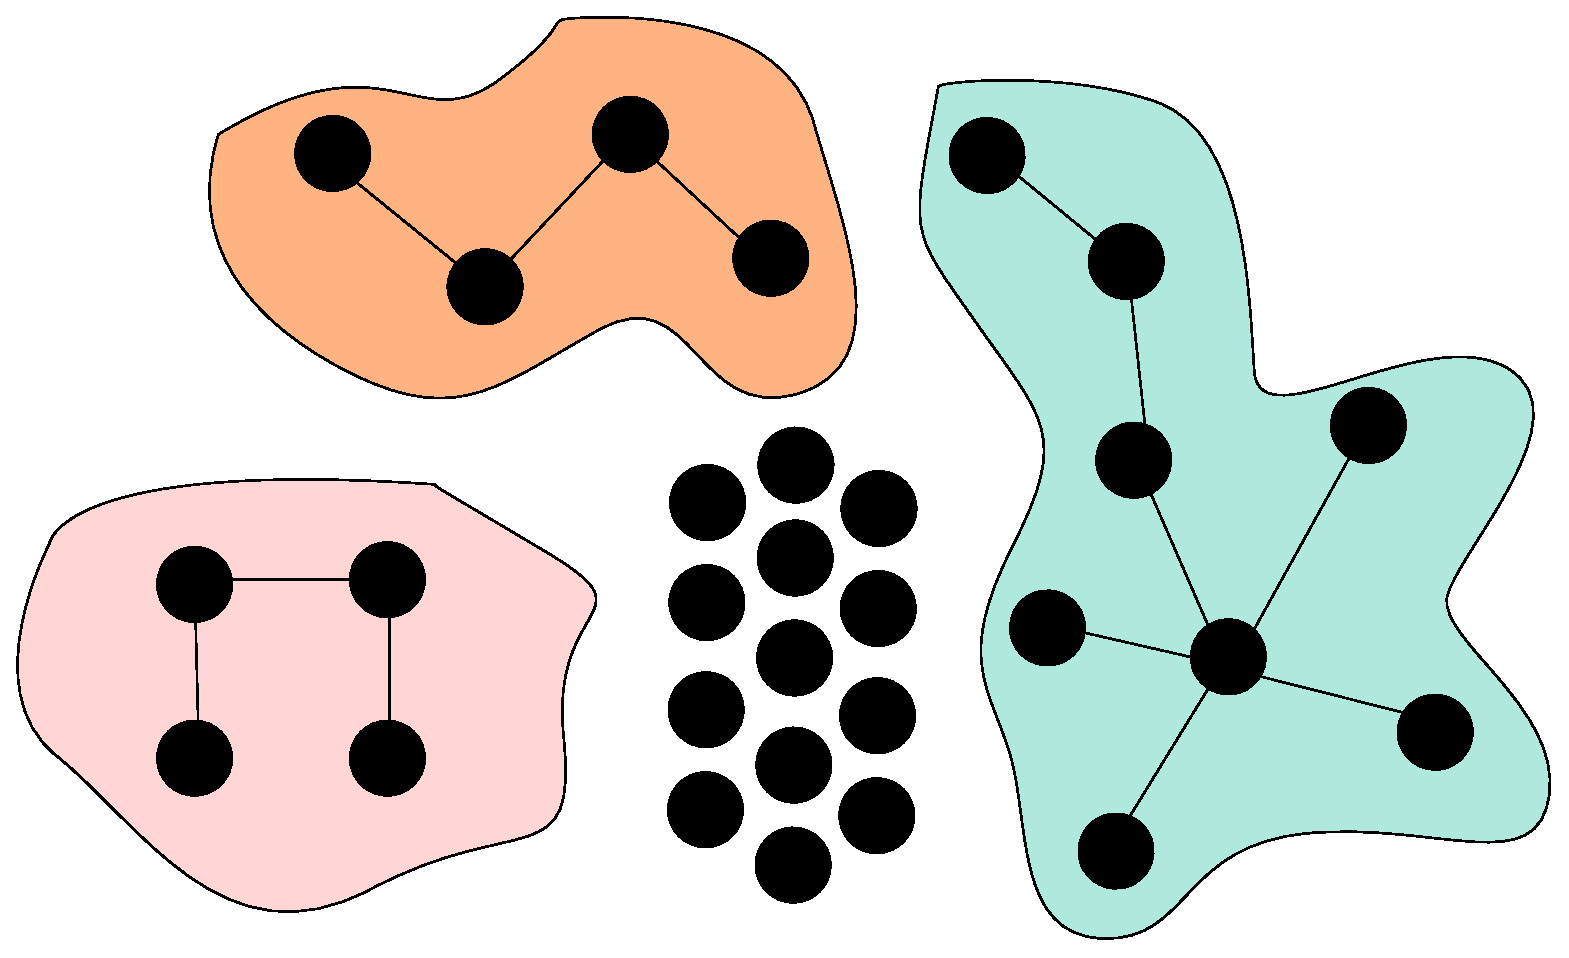
\includegraphics[width=\textwidth]{transitiveclosure}
Clustering topics (black dots) by Transitive Closure based on similarity (arcs)
\end{center}


\newslide

\begin{table*}
\centering
\begin{tabular}{|ccc|l|}

%\hline
%2000 &  Jul &  31 &    chmod \\
%2000 &  Sep &  29 &    fixes benchmark logging windows \\
%2000 &  Nov &  28 &    typo fix insert\_multi\_value \\
%2001 &  Jan &  27 &    fixes Innobase Cleanups auto-union \\
%2001 &  Mar &  28 &    2 topics bugfix, logging , TEMPORARY,  \\
\hline
2001 &  Jul &  26 &    update Allow TABLES LOCK [a] \\ 

2001 &  Aug &  25 &    tables row version [a] \\
\hline
%2001 &  Sep &  24 &    update checksum merge \\
%2001 &  Oct &  24 &    fixed fix \\
%2001 &  Dec &  23 &    HPUX SCO fix \\
\hline
2002 &  Feb &  21 &    net buffer length  max\_allowed\_packet [b] \\
2002 &  Mar &  23 &    small buf fix [b]  \\
%\hline
%2002 &  May &  22 &    [popular] fix SCO OSF1 table\_name \\
%2002 &  Nov &  18 &    HPUX11 compiler HP \\
\hline
\hline
2003 &  Feb &  16 &    Linux errno  [c] \\
2003 &  Mar &  18 &    alarm bookmark bug [c] \\
%\hline
%2003 &  Sep &  14 &    Auto logging merge windows distribution fix 64-bit 4.0 Cleanup \\
\hline
\end{tabular}
\caption{Continuous blocks found while tracking topics associated with the word portability in MySQL 3.23}
\label{tab:portability}
\end{table*}

\newslide

% \begin{figure}
%   \centering
%   \includegraphics[width=1.5\textwidth]{lda}
%   \caption{Example of topics extracked from MySQL 3.23}
%   \label{fig:mysql323}
% \end{figure}

\igbigslidecap{lda}{Example of topics extracted from MySQL 3.23}

=
\end{slide}


\end{document}
